\begin{objectives}
	In this tutorial you will characterize first order differential equations.
\end{objectives}

\subsection*{Problems}
\begin{enumerate}
\item Draw a phase plot (plot of $y$ vs., $f(y)$) for an autonomous ODE $y'=f(y)$ such that:
\begin{itemize}[nosep]
	\item The ODE has three equilibria.
	\item At least one of the equilibria is stable.
	\item \textbf{NONE} of the equilibria are unstable.
\end{itemize}
Explain and justify that your phase plot does actually fulfill these requirements.

\item Consider the following ODEs. Are they linear or not? Are they separable or not?
\begin{tcolorbox}[sharp corners=all,colframe=tolGrey,colback=white]
    \begin{multicols}{2}
    \begin{enumerate}[label={(\roman{enumii})},nosep,itemsep=1mm]
        \item $y'=t^2y$
        \item $y'=t\sin y$
        \item $y'=y\sin t$
        \item $y'=t+\sin y$
        \item $y'=y+\sin t$
        \item $y'=y(t^2+1)$
        \item $y'=e^{2t-y}$
        \item $y'-2y=3e^t$
        \item $y'e^{t/2}=y^2+4$
        \item $y'+y=5\sin 2t$
    \end{enumerate}
    \end{multicols}
\end{tcolorbox}

\item Consider the below ODEs and problem descriptions. Match each ODE to a problem description and justify your answer.
\begin{tcolorbox}[sharp corners=all,colframe=tolGrey,colback=white]
    \begin{multicols}{2}
    \begin{enumerate}[label={(\roman{enumii})},nosep,itemsep=1mm]
        \item $y'=ky$
        \item $y'=ky(M-y)$
        \item $y'=\frac{ky(M-y)}{\sqrt{t+1}}$
    \end{enumerate}
    \end{multicols}
\end{tcolorbox}

Consider the below descriptions:
\begin{enumerate}
    \item Babies are born on an island at a constant rate, but there is a carrying capacity which limits the number of people that the island can support.
    \item Babies are born on an island at a constant rate.
    \item Babies are born on an island at a constant rate, but as time progresses, people become more rich and have fewer children.
\end{enumerate}

% \begin{minipage}[t]{\linewidth-7cm}
% \item Consider the ODE
% \[
%     \frac{\mathrm dy}{\mathrm dt} = f(y) = (y-1)^2 (y-2) (y-3)
% \]
% The phase plot of this ODE is given on the right.

% \textit{You can answer this question based on the equation, the phase plot, or both!}
% \begin{enumerate}
% \item Find and classify the equilibrium points of the differential equation. Make sure to justify your answer.
% \vspace{3mm}

% \item If $y(t)$ is a solution to the ODE, and $y(0.5)=2.8$, what is $\lim_{t\to\infty} y(t)$? Justify your choice.
% \end{enumerate}
% \end{minipage}\hfill
% \begin{minipage}[t]{6cm}
% 	\vfil
% 	\vspace{-6mm}
% 	\flushright
% 	\begin{tikzpicture}[line width=1]
% 		\draw [black!20] (-0.5,-1) grid [step=0.5] (4,3);
% 		\begin{scope}
% 		\clip (0,-1) rectangle (4,3);
% 		\draw [smooth,samples=100,domain=0:3.5,tolOrange] plot ({\x},{(\x-1)*(\x-1)*(\x-2)*(\x-3)});
% 		\end{scope}
% 	\draw [->] (-0.5,0) -- (4,0) node [right] {$y$};
% 	\draw [->] (0,-1) -- (0,3) node [above] {$f(y)$};
% 	\draw (1,0.1) -- (1,-0.1) node [below] {1};
% %	\draw (0.1,1) -- (-0.1,1) node [left] {1};
% \end{tikzpicture}
% \end{minipage}

% \clearpage
% \item Match the direction fields below with the following ODEs. There are more ODEs than figures, so some won't have a match. Make sure to provide an argument in words justifying the matching.
% \begin{multicols}{2}
%     \begin{enumerate}[label={(\roman{enumii})},nosep,itemsep=1mm]
%         \item $y'=2y-1$
%         \item $y'=2+y$
%         \item $y'=y-2$
%         \item $y'=y(y+3)$
%         \item $y'=y(y-3)$
%         \item $y'=1+2y$
%         \item $y'=-2-y$
%         \item $y'=y(3-y)$
%         \item $y'=1-2y$
%         \item $y'=2-y$
%     \end{enumerate}
%     \end{multicols}

% 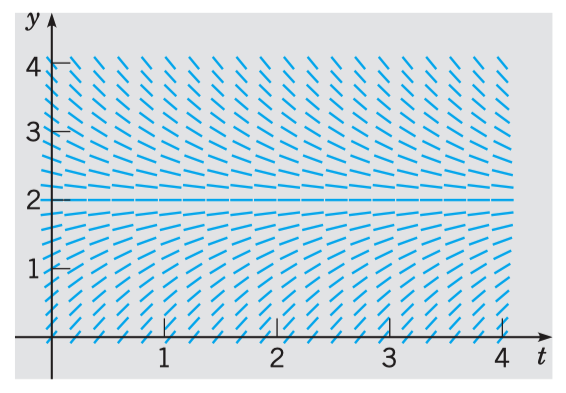
\includegraphics[width=0.4\linewidth]{field1}
% 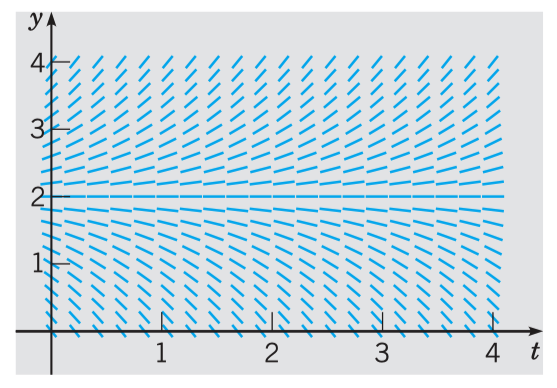
\includegraphics[width=0.4\linewidth]{field2}\\
% \null\hfill\textbf{(A)}\hfill\hfill
% \textbf{(B)}\hfill
% \null

% \vspace{3mm}
% \hrule

% 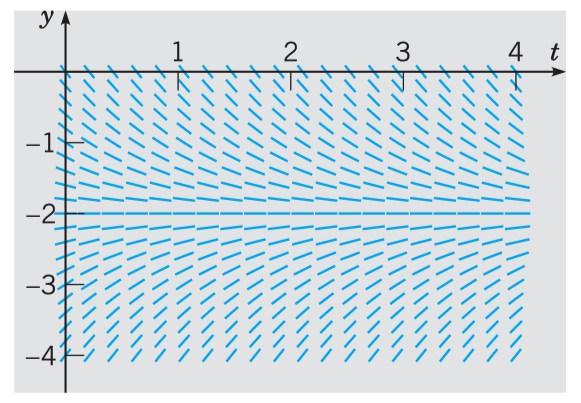
\includegraphics[width=0.4\linewidth]{field3}
% 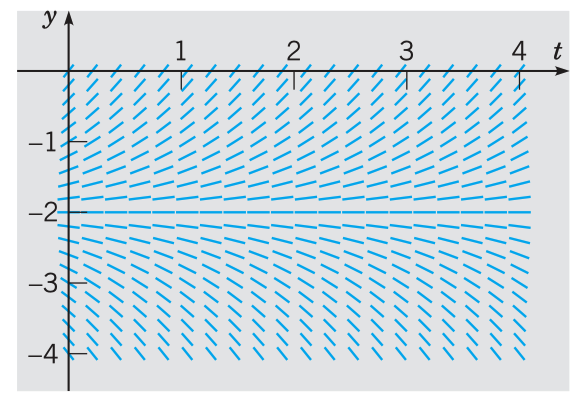
\includegraphics[width=0.4\linewidth]{field4}\\
% \null\hfill\textbf{(C)}\hfill\hfill
% \textbf{(D)}\hfill
% \null

% \vspace{3mm}
% \hrule

% 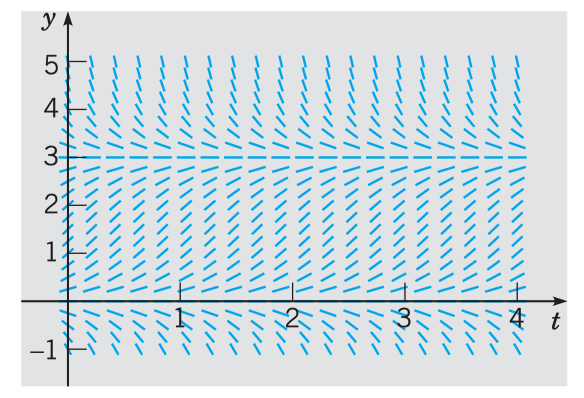
\includegraphics[width=0.4\linewidth]{field5}
% 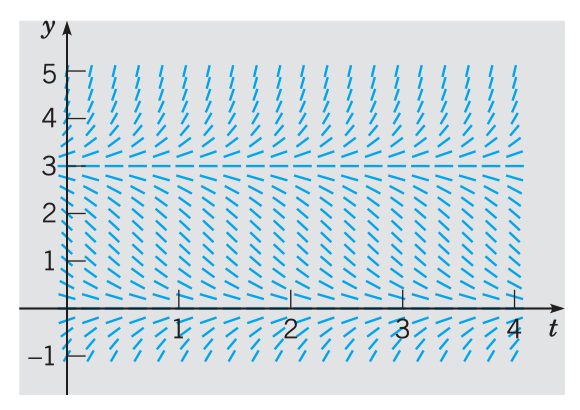
\includegraphics[width=0.4\linewidth]{field6}\\
% \null\hfill\textbf{(E)}\hfill\hfill
% \textbf{(F)}\hfill
% \null
% \clearpage

% \item We will attempt to model how people leave a soccer stadium at the end of a game. We define the radius of the populated area in the stadium around an exit as $r(t)$. $t$ is the time in minutes and our observation starts at $t=0$.
	
% 	The flow of people will obey Torricelli’s Law which states that \textit{the area of the region occupied by people will decrease at a rate proportional to the square root of the radius and also proportional to the size of the exit}.
	
% 	\begin{enumerate}
% 	\begin{minipage}[t]{0.50\linewidth} 
%     	\item Use this to create an ODE that models the size of the crowd exiting the stadium. Introduce parameters as necessary.\medskip
    	
%     	\item Classify the ODE from the last part (order, linearity, separability etc.). Without solving the ODE, consider each parameter and each variable: What are its units? How does it affect the behaviour of the ODE? How is the behaviour of this system affected if it is very large? very small? zero?\medskip

        
        
%         \item Find the general solution to the ODE. What is the solution if $r(0)=3$?
%     	\end{minipage}\hfill
%     	\begin{minipage}[t]{0.33\textwidth} 
%     	\vfil
%             \begin{flushright}
%             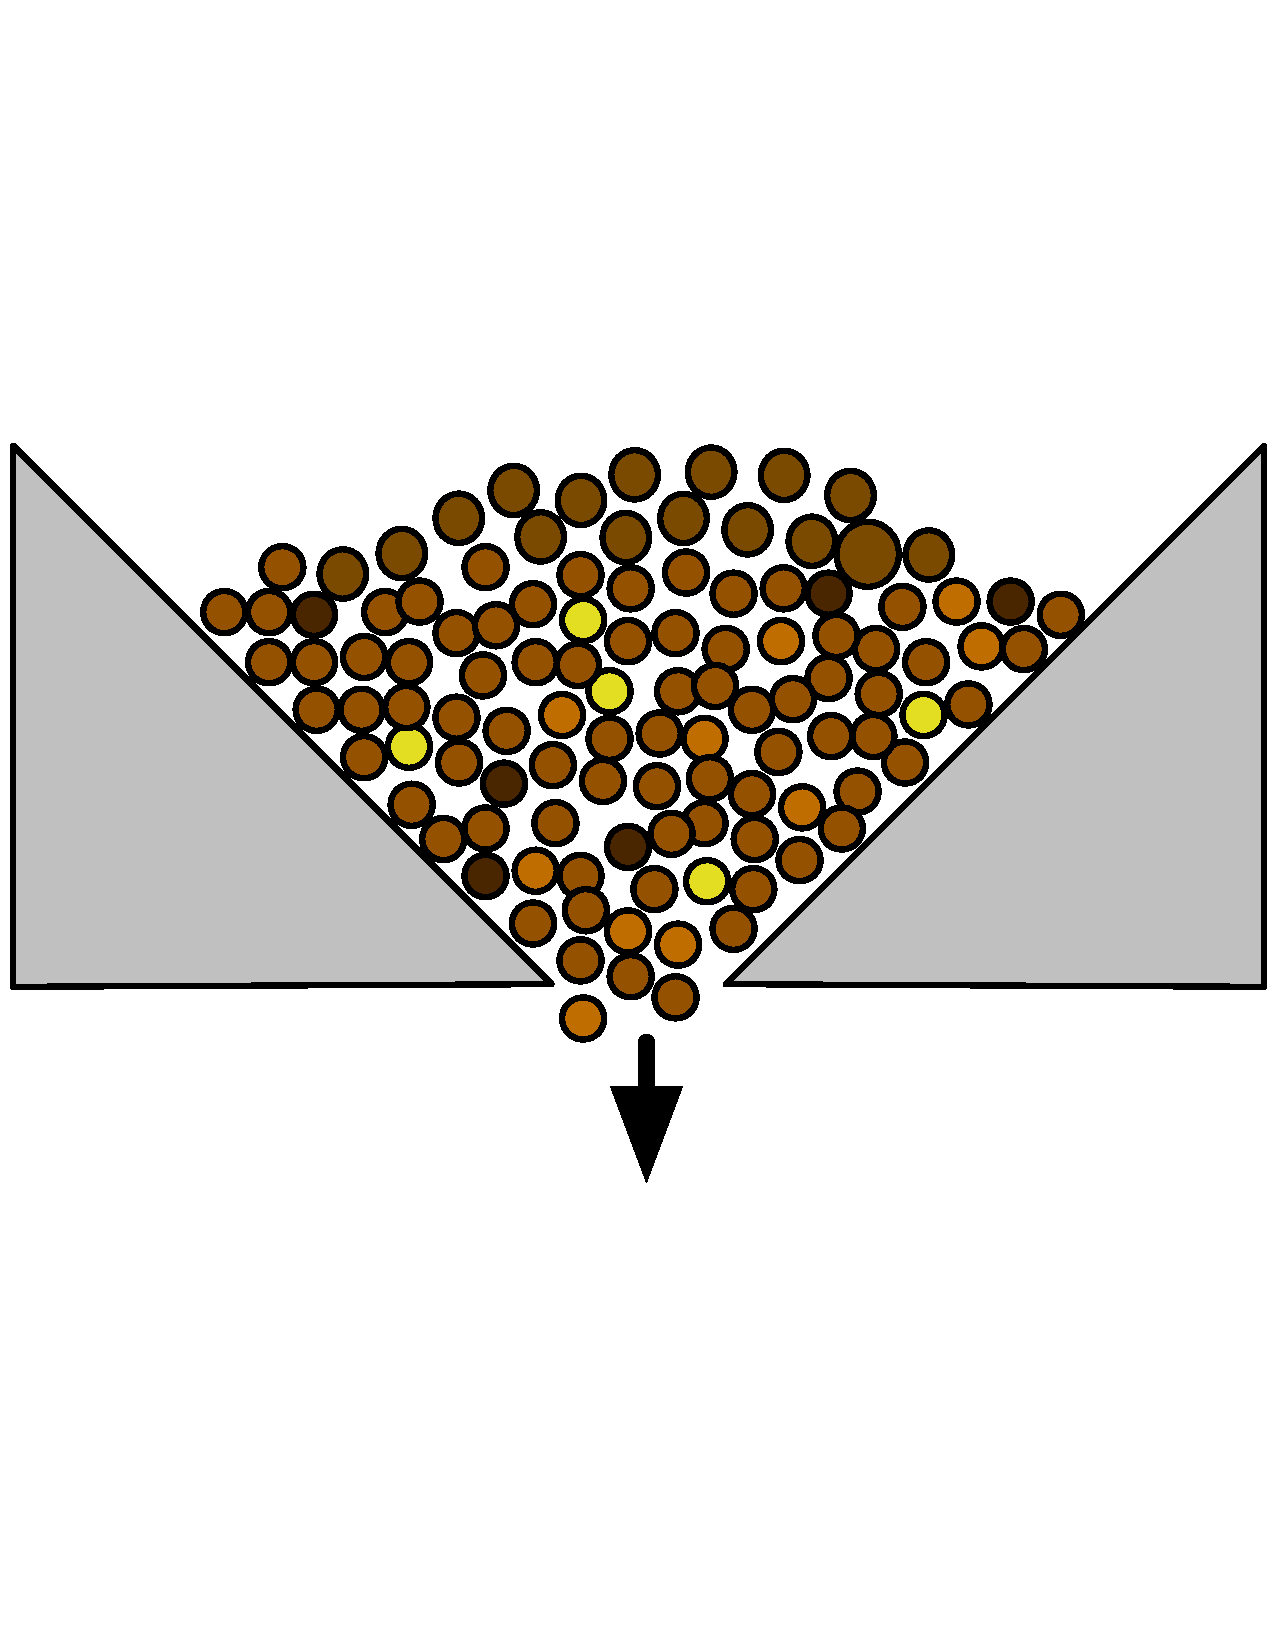
\includegraphics[width=1.0\textwidth]{stadium_fixed.pdf}\\
%             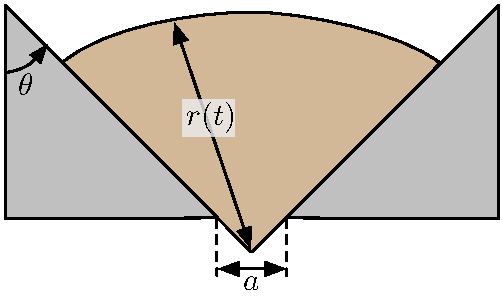
\includegraphics[width=1.0\textwidth]{stadium2.pdf}    
%             \end{flushright}
%         \end{minipage}
%     \end{enumerate}
\end{enumerate}
